\documentclass[12pt,]{tufte-handout}

% ams
\usepackage{amssymb,amsmath}

\usepackage{ifxetex,ifluatex}
\usepackage{fixltx2e} % provides \textsubscript
\ifnum 0\ifxetex 1\fi\ifluatex 1\fi=0 % if pdftex
  \usepackage[T1]{fontenc}
  \usepackage[utf8]{inputenc}
\else % if luatex or xelatex
  \makeatletter
  \@ifpackageloaded{fontspec}{}{\usepackage{fontspec}}
  \makeatother
  \defaultfontfeatures{Ligatures=TeX,Scale=MatchLowercase}
  \makeatletter
  \@ifpackageloaded{soul}{
     \renewcommand\allcapsspacing[1]{{\addfontfeature{LetterSpace=15}#1}}
     \renewcommand\smallcapsspacing[1]{{\addfontfeature{LetterSpace=10}#1}}
   }{}
  \makeatother

    \setmainfont[]{Tw Cen MT}
\fi

% graphix
\usepackage{graphicx}
\setkeys{Gin}{width=\linewidth,totalheight=\textheight,keepaspectratio}

% booktabs
\usepackage{booktabs}

% url
\usepackage{url}

% hyperref
\usepackage{hyperref}

% units.
\usepackage{units}


\setcounter{secnumdepth}{-1}

% citations


% pandoc syntax highlighting

% longtable
\usepackage{longtable,booktabs}

% multiplecol
\usepackage{multicol}

% strikeout
\usepackage[normalem]{ulem}

% morefloats
\usepackage{morefloats}


% tightlist macro required by pandoc >= 1.14
\providecommand{\tightlist}{%
  \setlength{\itemsep}{0pt}\setlength{\parskip}{0pt}}

% title / author / date
\title{Data Driven Report Demo}
\author{Andrew Grogan-Kaylor}
\date{2021-04-13}


\begin{document}

\maketitle




\hypertarget{background}{%
\section{Background}\label{background}}

Life expectancy differs in countries around the world. Life expectancy
and \emph{per capita} \emph{Gross Domestic Product} (GDP) appear to be
related.

\begin{marginfigure}
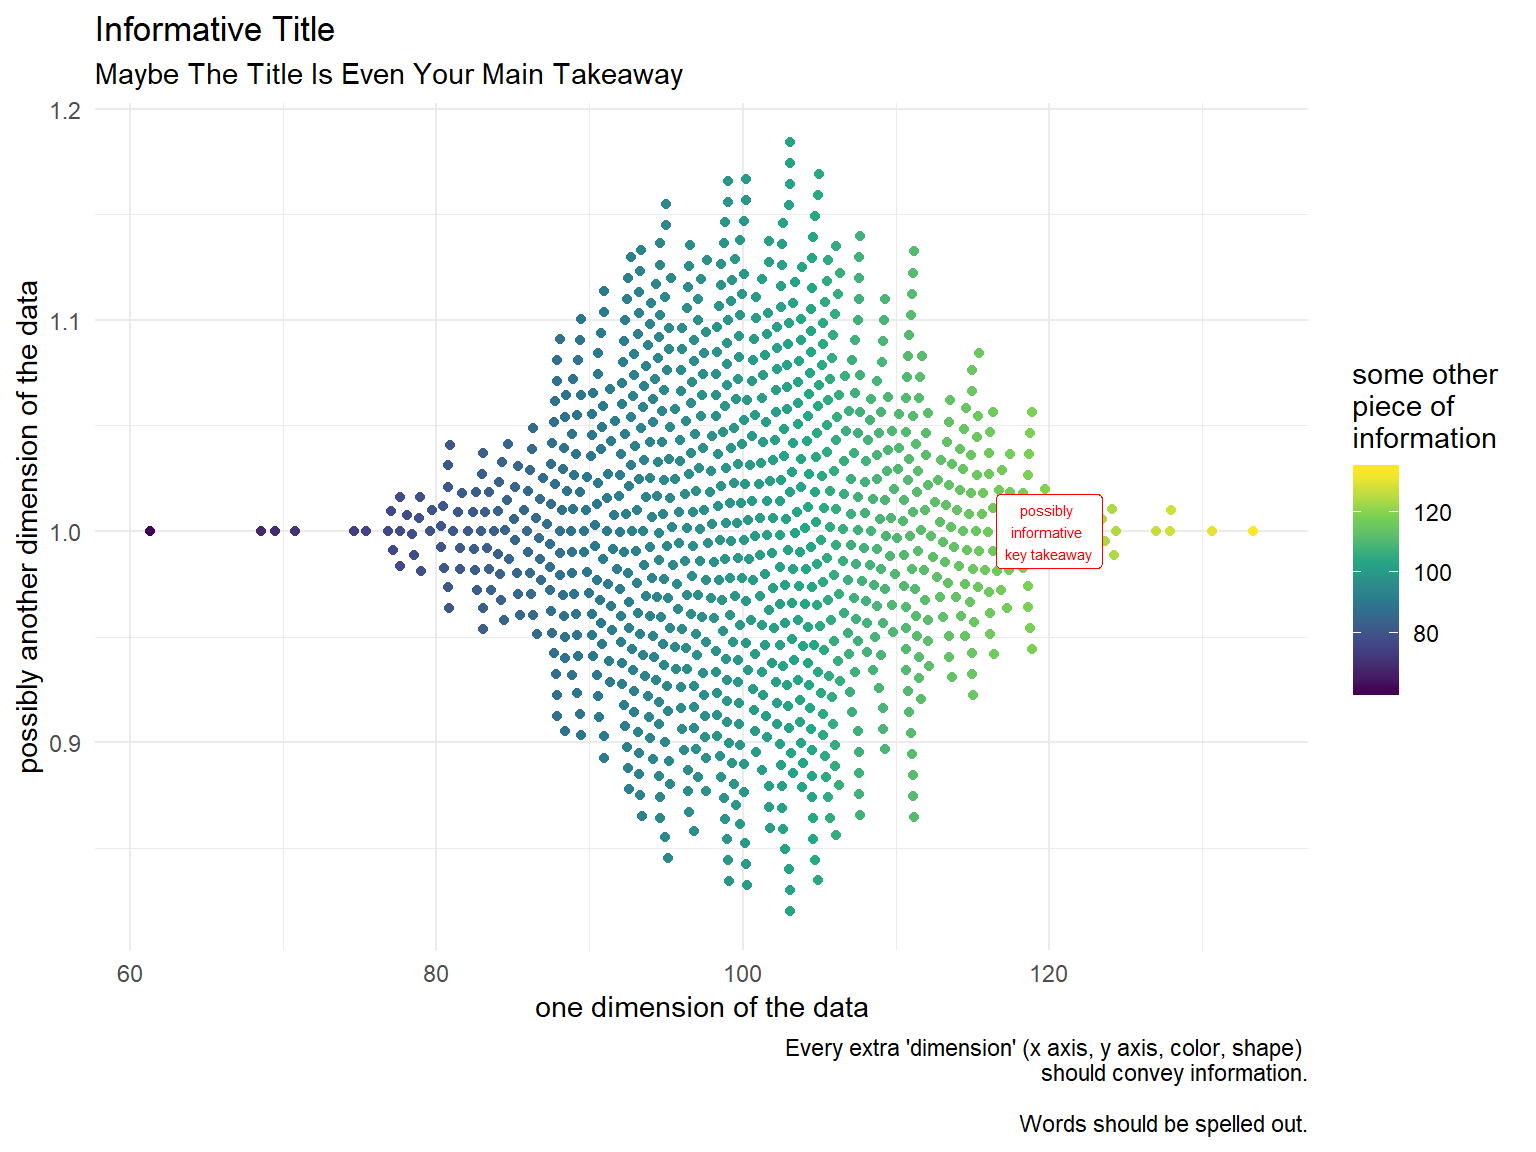
\includegraphics{data-driven-report-demo-tufte_files/figure-latex/unnamed-chunk-2-1} \end{marginfigure}

\hypertarget{methods}{%
\section{Methods}\label{methods}}

Data were provided via the \texttt{gapminder} library which provides a
sample of data available on
\href{http://www.gapminder.org}{gapminder.org}

\hypertarget{results}{%
\section{Results}\label{results}}

Results indicate the per capita GDP and life expectancy are related in a
non-linear way.

\begin{marginfigure}
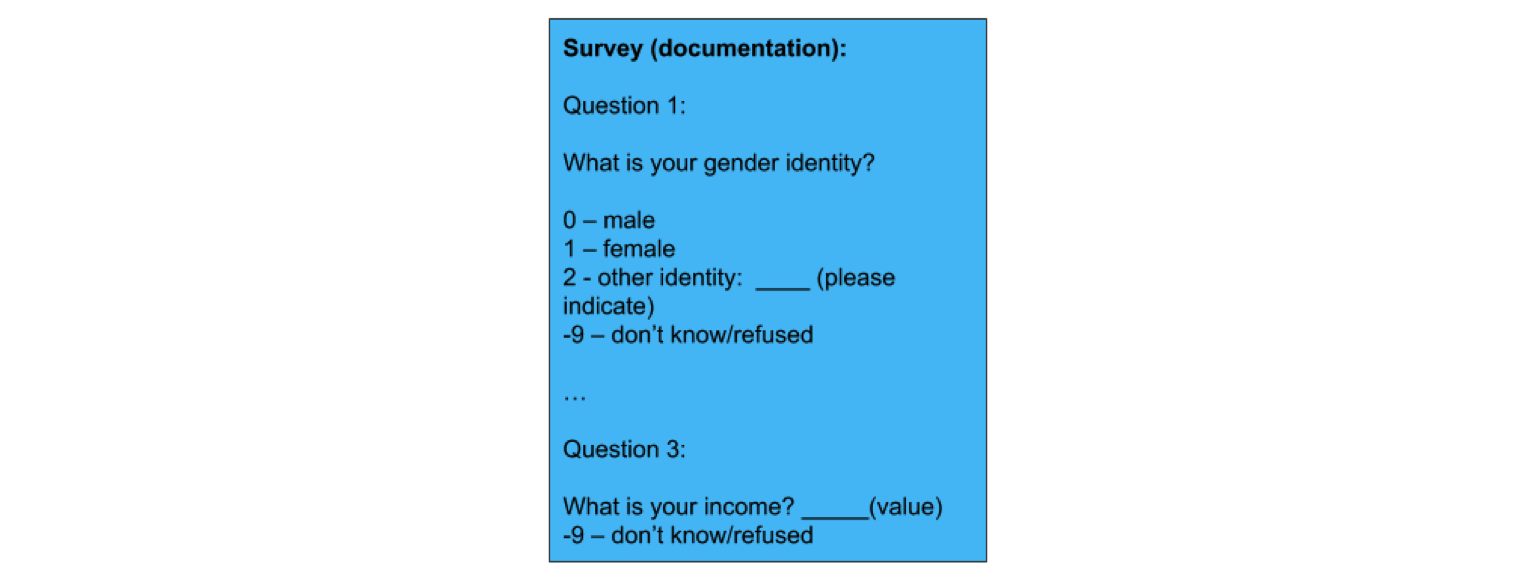
\includegraphics{data-driven-report-demo-tufte_files/figure-latex/unnamed-chunk-3-1} \end{marginfigure}

\begin{longtable}[]{@{}
  >{\centering\arraybackslash}p{(\columnwidth - 10\tabcolsep) * \real{0.10}}
  >{\centering\arraybackslash}p{(\columnwidth - 10\tabcolsep) * \real{0.14}}
  >{\centering\arraybackslash}p{(\columnwidth - 10\tabcolsep) * \real{0.12}}
  >{\centering\arraybackslash}p{(\columnwidth - 10\tabcolsep) * \real{0.11}}
  >{\centering\arraybackslash}p{(\columnwidth - 10\tabcolsep) * \real{0.14}}
  >{\centering\arraybackslash}p{(\columnwidth - 10\tabcolsep) * \real{0.10}}@{}}
\caption{Life Expectancy}\tabularnewline
\toprule
Min. & 1st Qu. & Median & Mean & 3rd Qu. & Max. \\
\midrule
\endfirsthead
\toprule
Min. & 1st Qu. & Median & Mean & 3rd Qu. & Max. \\
\midrule
\endhead
23.6 & 48.2 & 60.71 & 59.47 & 70.85 & 82.6 \\
\bottomrule
\end{longtable}

\begin{longtable}[]{@{}
  >{\centering\arraybackslash}p{(\columnwidth - 10\tabcolsep) * \real{0.11}}
  >{\centering\arraybackslash}p{(\columnwidth - 10\tabcolsep) * \real{0.14}}
  >{\centering\arraybackslash}p{(\columnwidth - 10\tabcolsep) * \real{0.12}}
  >{\centering\arraybackslash}p{(\columnwidth - 10\tabcolsep) * \real{0.10}}
  >{\centering\arraybackslash}p{(\columnwidth - 10\tabcolsep) * \real{0.14}}
  >{\centering\arraybackslash}p{(\columnwidth - 10\tabcolsep) * \real{0.14}}@{}}
\caption{GDP Per Capita}\tabularnewline
\toprule
Min. & 1st Qu. & Median & Mean & 3rd Qu. & Max. \\
\midrule
\endfirsthead
\toprule
Min. & 1st Qu. & Median & Mean & 3rd Qu. & Max. \\
\midrule
\endhead
241.2 & 1202 & 3532 & 7215 & 9325 & 113523 \\
\bottomrule
\end{longtable}

\hypertarget{discussion}{%
\section{Discussion}\label{discussion}}

\emph{Per capita} GDP and life expectancy appear to be related. These
findings may have implications for public health policy, for development
policy, for intervention, and for advocacy.



\end{document}
